\documentclass[12pt]{article}

% URLs and hyperlinks ---------------------------------------
\usepackage{hyperref}
\hypersetup{
	colorlinks=true,
	linkcolor=blue,
	filecolor=magenta,      
	urlcolor=blue,
}
\usepackage{xurl}
%---------------------------------------------------

\usepackage{float}
\usepackage{adjustbox}
\usepackage{graphicx}
\usepackage{rotating}
\usepackage{mathtools}
\usepackage{enumitem}
\usepackage{gensymb}

\usepackage{xepersian}
\settextfont{Yas}

\title{گزارش کار آزمایش نهم}
\author{	گروه: \\	اریسا احسانی \\	سید حسین حسینی \\	مهدی حق‌وردی \\ \\	شعبه شش
}
\date{}
\renewcommand{\arraystretch}{1.4}

\begin{document}
\maketitle
\tableofcontents
\clearpage

\section{1}

\begin{latin}
\begin{table}[H]
\begin{center}
\begin{tabular}{|c|c|c|c|}
\hline
\rl{جنس} & NPN or PNP & \rl{شکل‌ ظاهری و پایه‌ها} & \rl{شماره ترانزیستور} \\
\hline
\hline
Si & NPN & \rl{استوانه‌ای} & 2N1711 \\
\hline
Si & PNP & \rl{استوانه‌ای} & 2N2905 \\
\hline
Si & NPN & \rl{استوانه‌ای} & 2N2369 \\
\hline
\end{tabular}
\end{center}
\end{table}
\end{latin}

\begin{figure}[H]
	\begin{center}
		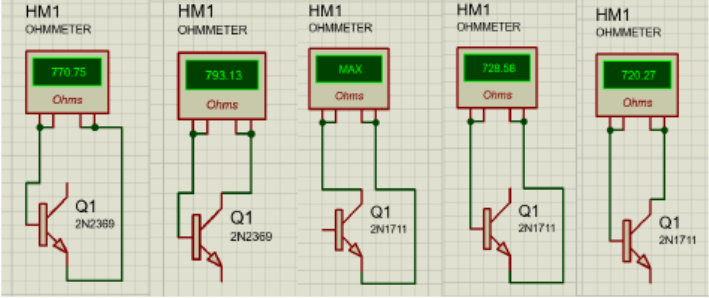
\includegraphics[width=\textwidth, height=6cm]{./images/9.1}
	\end{center}
\end{figure}

\begin{figure}[H]
	\begin{center}
		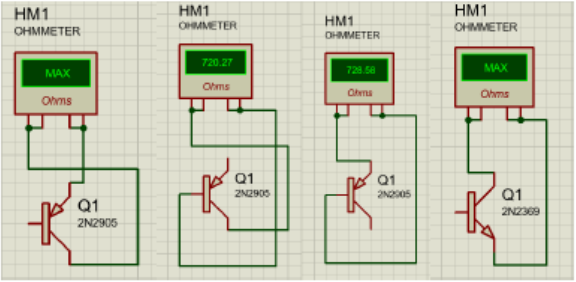
\includegraphics[width=\textwidth, height=6cm]{./images/9.2}
	\end{center}
\end{figure}

\clearpage
\section{2}
در حالت \lr{NPN}:
\begin{figure}[H]
	\begin{center}
		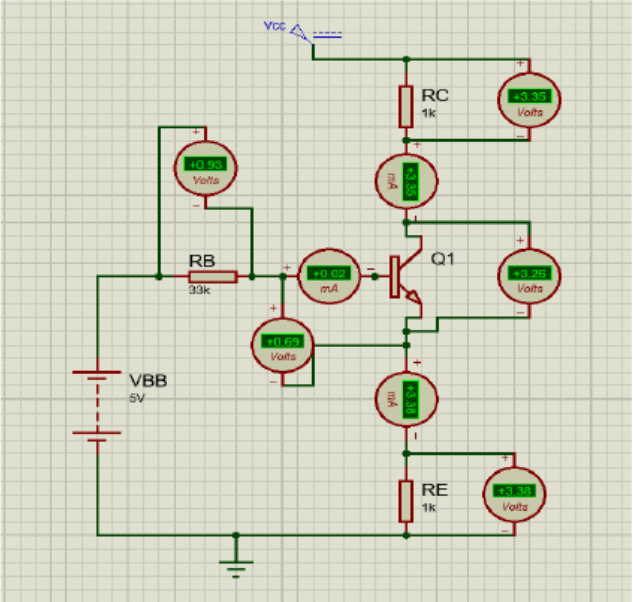
\includegraphics[width=\textwidth, height=12cm]{./images/9.3}
	\end{center}
\end{figure}

\begin{figure}[H]
	\begin{center}
		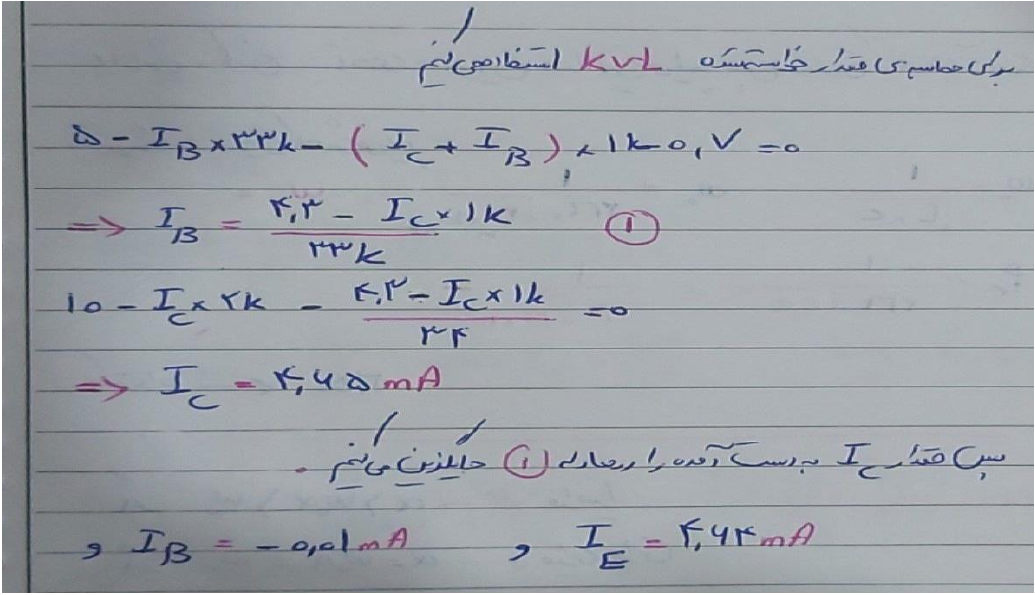
\includegraphics[width=\textwidth, height=11cm]{./images/9.3.1}
	\end{center}
\end{figure}

\begin{latin}
\begin{center}
\begin{tabular}{|c|c|c|c|}
\hline
\rl{پارامتر} & \rl{مقدار اندازه‌‌گیری شده} & \rl{مقدار محاسبه شده} & \rl{درصد خطا} \\
\hline
\hline
$V_c\ V$ & 6.65 & 5.35 & 20 \% \\
\hline
$V_b\ V$ & 4.07 & 5.33 & 30 \% \\
\hline
$V_e\ V$ & 3.38 & 4.63 & 37 \% \\
\hline
$I_{cq}\ mA$ & 3.35 & 4.65 & 38 \% \\
\hline
$I_{bq}\ mA$ & 0.02 & -0.01 & 50 \% \\
\hline
$I_{eq}\ mA$ & 3.38 & 4.64 & 37 \% \\
\hline
$\beta_{dc}$ & 167.5 & - & - \\
\hline
$V_{ceq}\ V$ & 3.26 & 0.72 & 78 \% \\
\hline
$V_{beq}\ V$ & 0.69 & 0.7 & 1 \% \\
\hline
\end{tabular}
\end{center}
\end{latin}

\begin{figure}[H]
	\begin{center}
		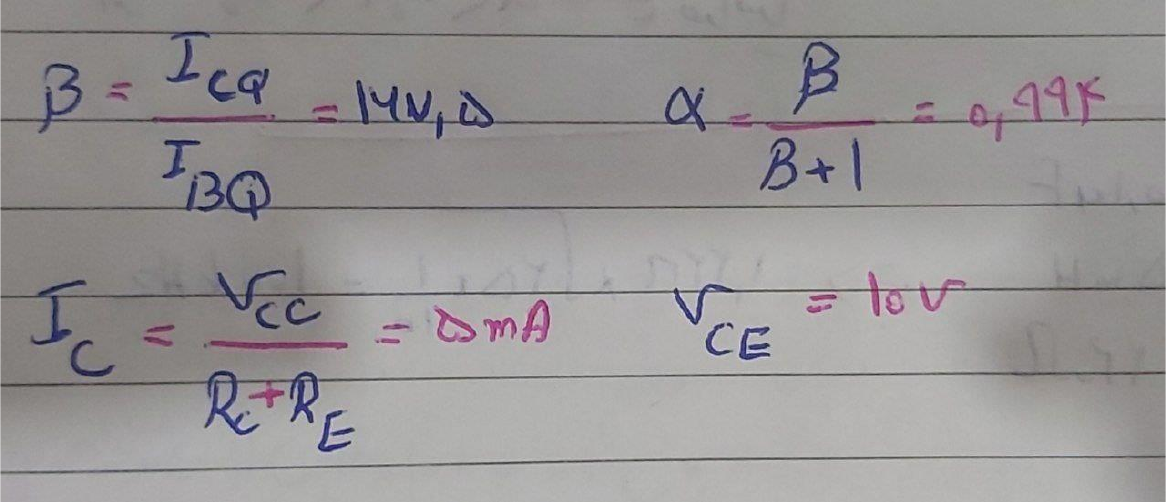
\includegraphics[width=\textwidth, height=6cm]{./images/9.3.2}
	\end{center}
\end{figure}
\begin{figure}[H]
	\begin{center}
		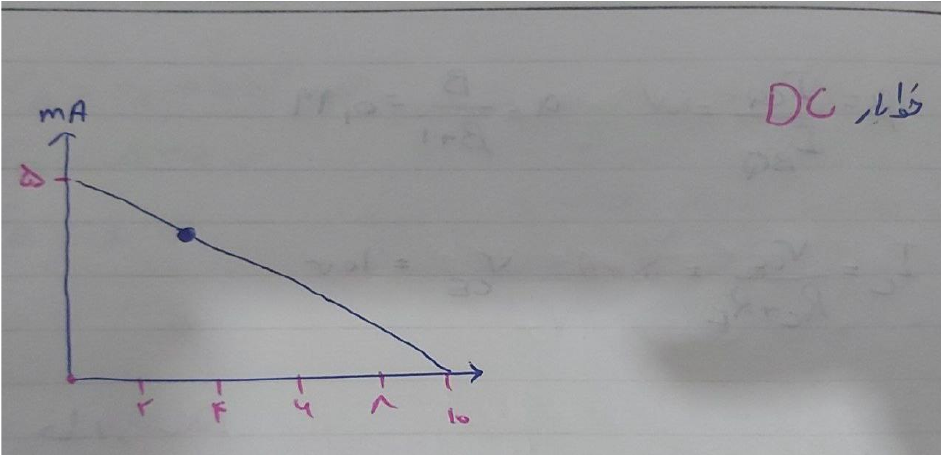
\includegraphics[width=\textwidth, height=6cm]{./images/9.3.3}
	\end{center}
\end{figure}

\clearpage
در حالت \lr{PNP}:
\begin{figure}[H]
	\begin{center}
		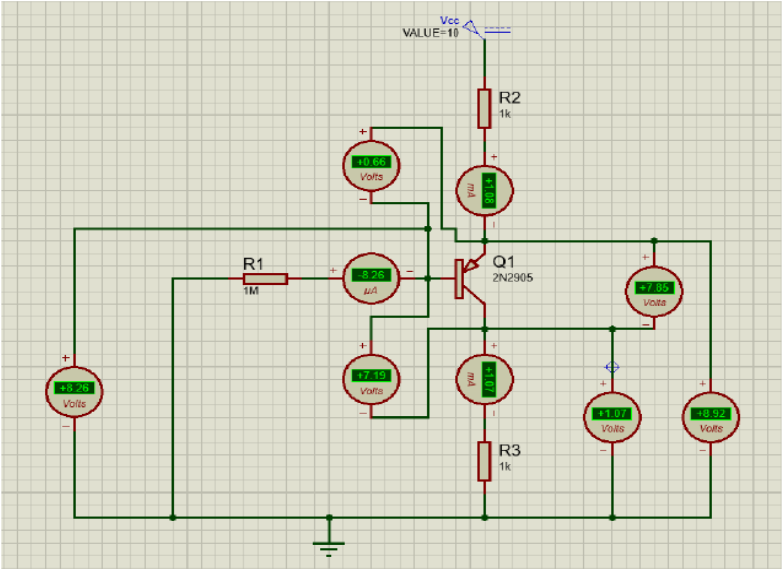
\includegraphics[width=\textwidth, height=12cm]{./images/9.4}
	\end{center}
\end{figure}

\begin{figure}[H]
	\begin{center}
		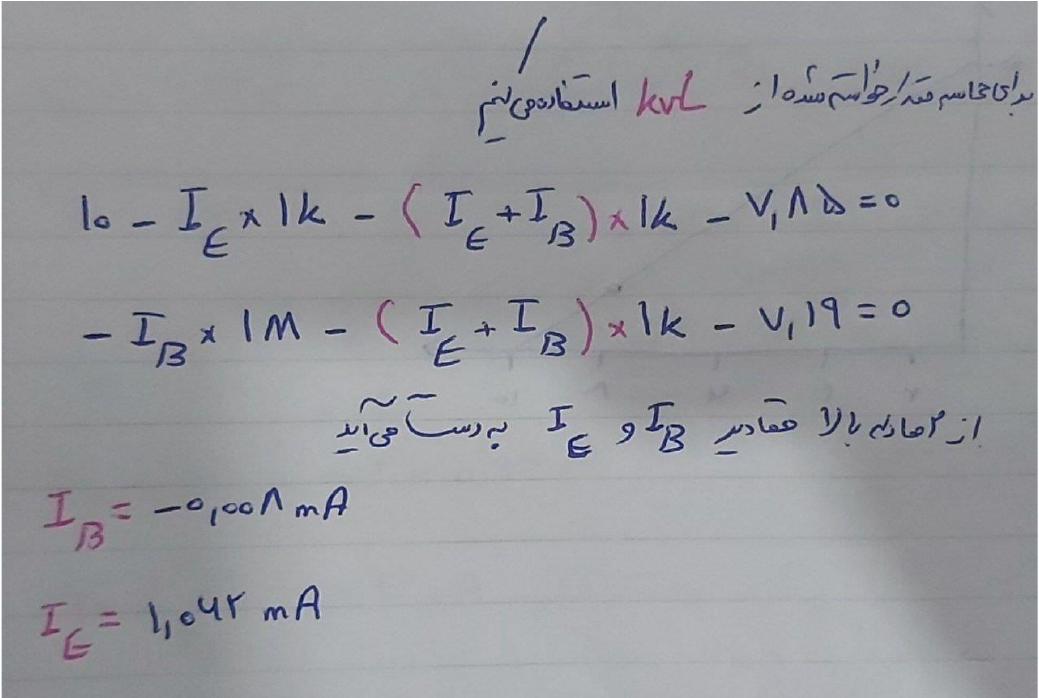
\includegraphics[width=\textwidth, height=11cm]{./images/9.4.1}
	\end{center}
\end{figure}

\begin{latin}
\begin{center}
\begin{tabular}{|c|c|c|c|}
\hline
\rl{پارامتر} & \rl{مقدار اندازه‌‌گیری شده} & \rl{مقدار محاسبه شده} & \rl{درصد خطا} \\
\hline
\hline
$V_c\ V$ & 1.07 & 1.062 & 1 \% \\
\hline
$V_b\ V$ & 8.26 & 8 & 4 \% \\
\hline
$V_e\ V$ & 8.92 & 8.93 & 0.1 \% \\
\hline
$I_{cq}\ mA$ & 1.07 & 1.062 & 1 \% \\
\hline
$I_{bq}\ mA$ & -0.01 & -0.008 & 25 \% \\
\hline
$I_{eq}\ mA$ & 1.08 & 1.07 & 1 \% \\
\hline
$\beta_{dc}$ & 107 & - & - \\
\hline
$V_{ceq}\ V$ & 7.85 & 7.868 & 0.2 \% \\
\hline
$V_{beq}\ V$ & 0.66 & 0.93 & 40 \% \\
\hline
\end{tabular}
\end{center}
\end{latin}

\begin{figure}[H]
	\begin{center}
		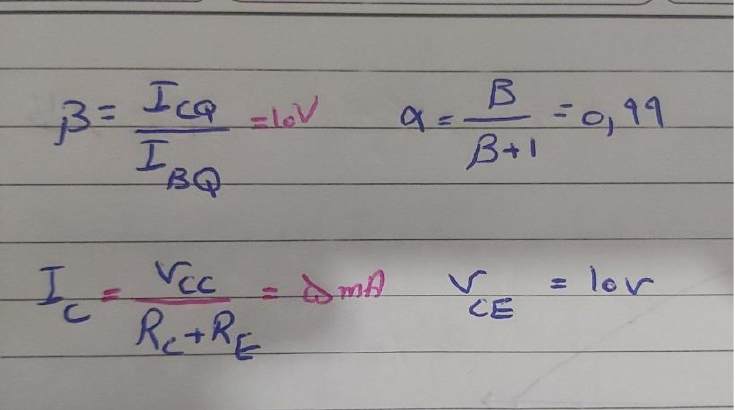
\includegraphics[width=\textwidth, height=6cm]{./images/9.4.2}
	\end{center}
\end{figure}
\begin{figure}[H]
	\begin{center}
		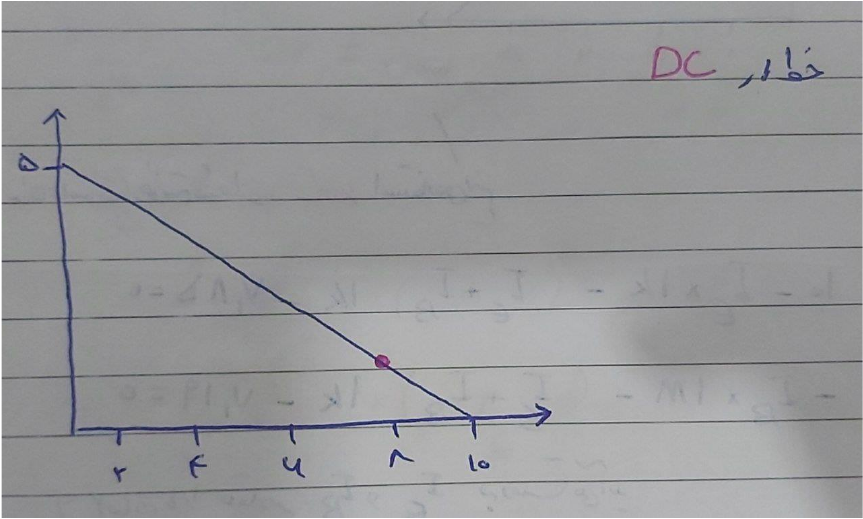
\includegraphics[width=\textwidth, height=6cm]{./images/9.4.3}
	\end{center}
\end{figure}

\clearpage
\section{3}
ابتدا مدار زیر را رسم می‌کنیم:
\begin{figure}[H]
	\begin{center}
		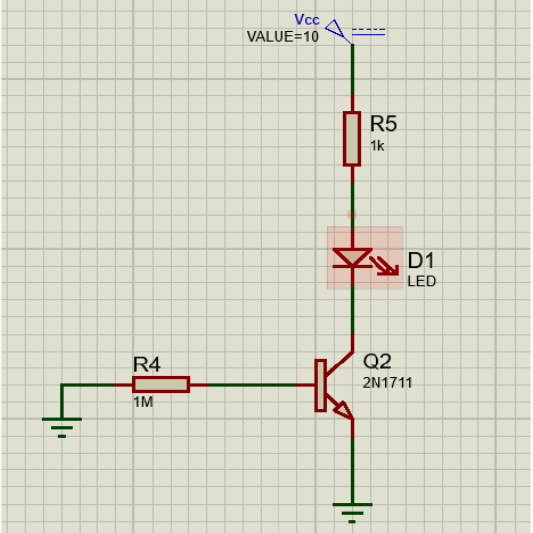
\includegraphics[width=0.7\textwidth, height=10cm]{./images/9.5}
	\end{center}
\end{figure}
\begin{figure}[H]
	\begin{center}
		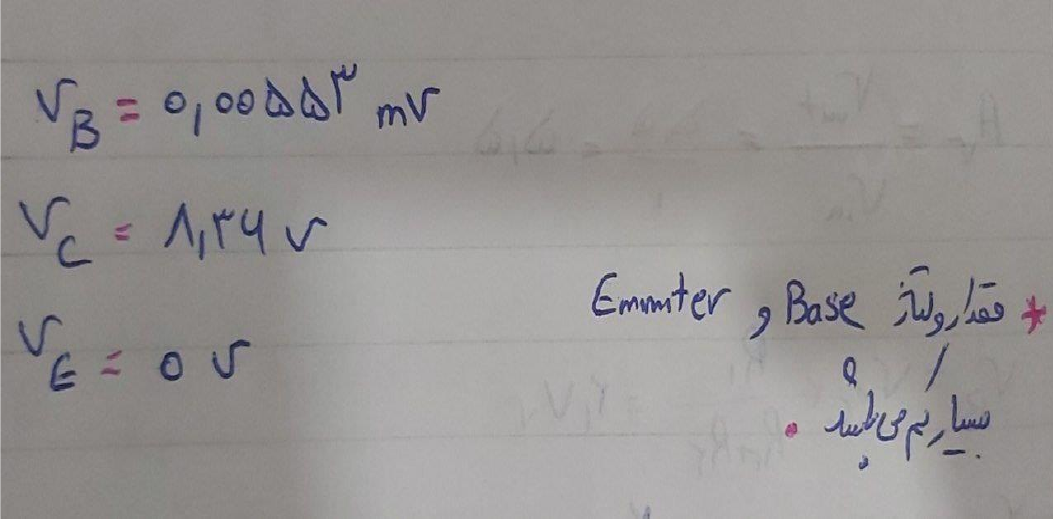
\includegraphics[width=\textwidth, height=6cm]{./images/9.5.1}
	\end{center}
\end{figure}

سپس به این صورت تغییر می‌دهیم:
\begin{figure}[H]
	\begin{center}
		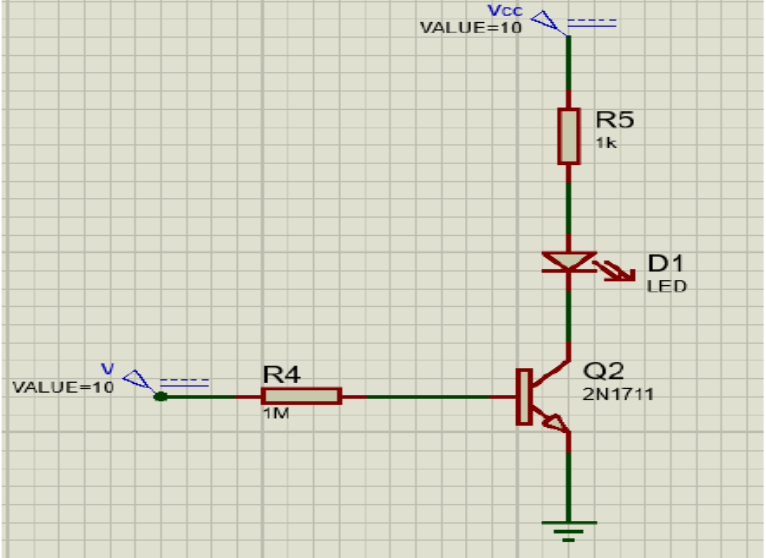
\includegraphics[width=0.7\textwidth, height=10cm]{./images/9.6}
	\end{center}
\end{figure}
\begin{figure}[H]
	\begin{center}
		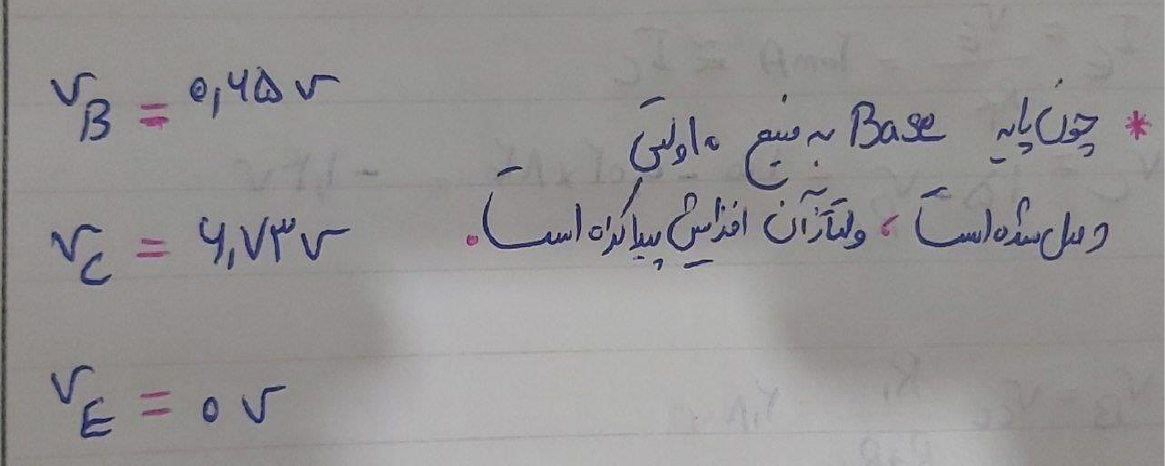
\includegraphics[width=\textwidth, height=6cm]{./images/9.6.1}
	\end{center}
\end{figure}

با توجه به اینکه پیوند بیس-امیتر مستقیم بایاس شده و پیوند بیس-کلکتور به صورت معکوس بایاس شده است، پس می‌توان گفت ترانزیستور‌ در حالت فعال است.

\clearpage
\section{4}

مدار:
\begin{figure}[H]
	\begin{center}
		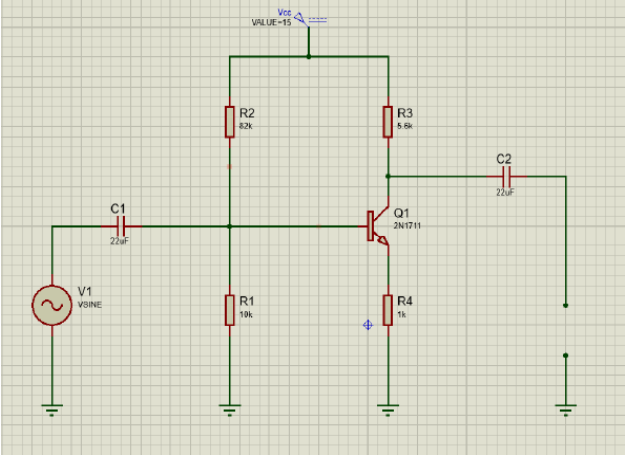
\includegraphics[width=\textwidth, height=8cm]{./images/9.7}
	\end{center}
\end{figure}

با حذف خازن‌‌ها داریم:
\begin{figure}[H]
	\begin{center}
		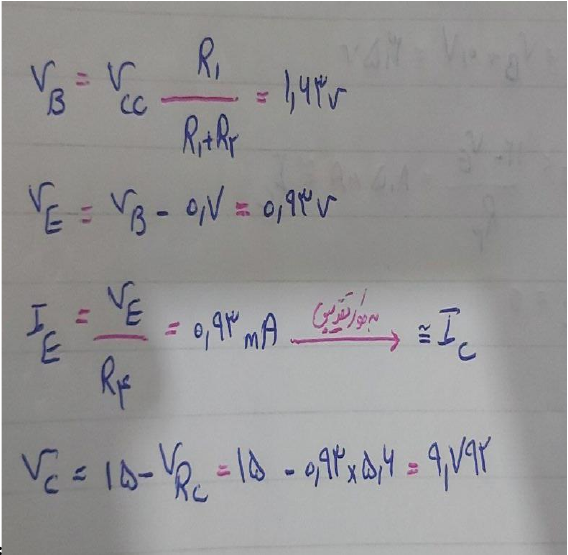
\includegraphics[width=\textwidth, height=5cm]{./images/9.7.1}
	\end{center}
\end{figure}

\begin{figure}[H]
	\begin{center}
		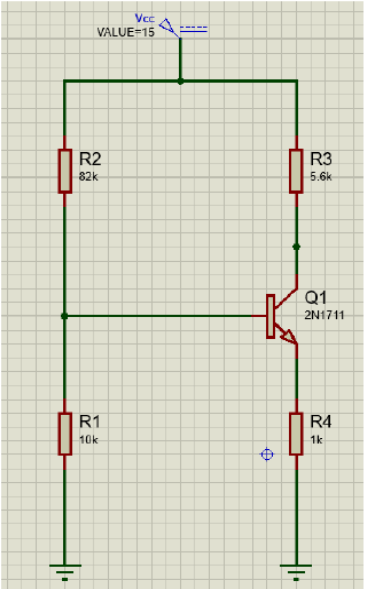
\includegraphics[width=0.7\textwidth, height=8cm]{./images/9.8}
	\end{center}
\end{figure}

سیگنال \lr{A} ورودی و سیگنال \lr{B} خروجی می‌باشد.
\begin{figure}[H]
	\begin{center}
		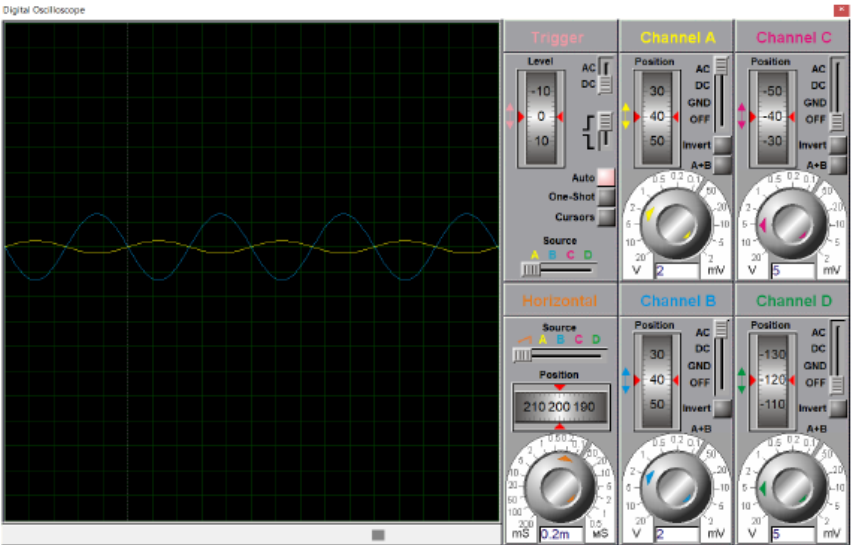
\includegraphics[width=\textwidth, height=8cm]{./images/9.9}
	\end{center}
\end{figure}

همانطور که انتظار داشتیم، اختلاف فاز ۱۸۰ درجه بین ورودی و خروجی وجود دارد. بهره‌ی ولتاژ این مدار برابر مقدار زیر است:

\begin{figure}[H]
	\begin{center}
		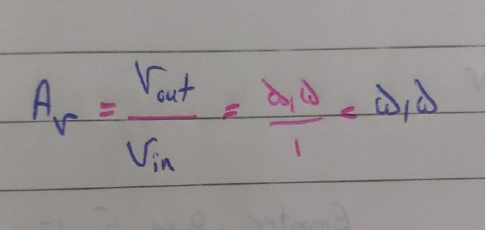
\includegraphics[width=\textwidth, height=6cm]{./images/9.7.2}
	\end{center}
\end{figure}

در صورتی که دامنه را روی $1.5$ قرار دهیم:

\begin{figure}[H]
	\begin{center}
		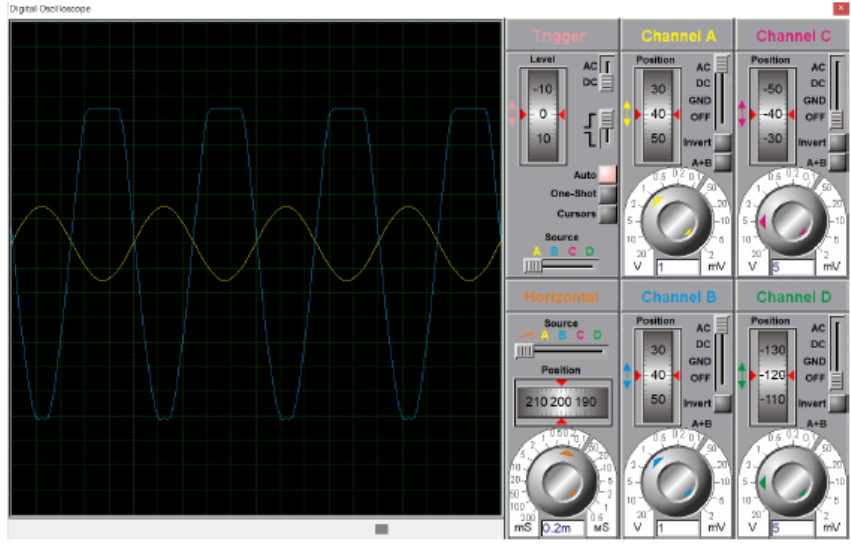
\includegraphics[width=\textwidth, height=6cm]{./images/9.10}
	\end{center}
\end{figure}

علت این برش‌ها این است که ترانزیستور قادر نیست سیگنال ورودی را تا بینهایت تقویت کند و آستانه‌ای دارد که این آستانه موجب برش سینگال خروجی می‌شود.

\clearpage
\section{5}
\begin{figure}[H]
	\begin{center}
		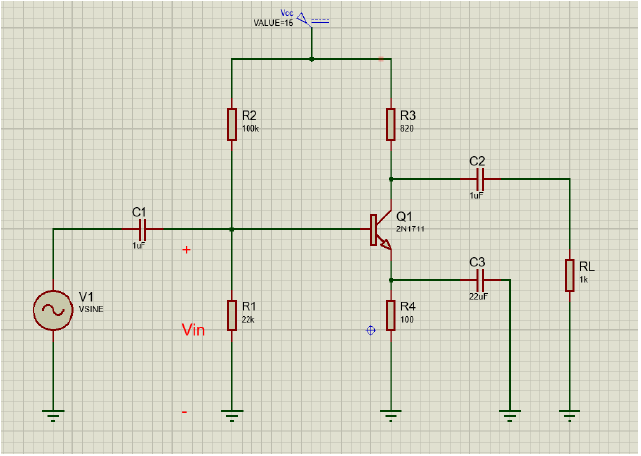
\includegraphics[width=\textwidth, height=6cm]{./images/9.11}
	\end{center}
\end{figure}

سیگنال ورودی را قطع و خازن‌ها را باز می‌کنیم:
\begin{figure}[H]
	\begin{center}
		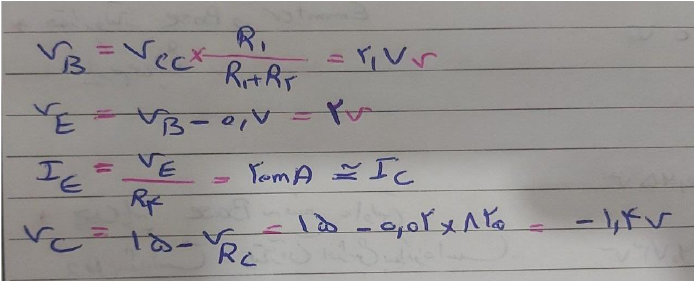
\includegraphics[width=\textwidth, height=6cm]{./images/9.11.1}
	\end{center}
\end{figure}


\begin{latin}
\begin{table}[H]
\begin{center}
\begin{tabular}{|c|c|c|}
\hline
DC \rl{پارامتر} & \rl{محاسبه شده} & \rl{اندازه‌گیری شده} \\
\hline
\hline
$V_B$ & 2.7 & 1.83 \\
\hline
$V_E$ & 2 & 1.09 \\
\hline
$I_E$ & 0.02 & - \\
\hline
$V_c$ & -1.4 & 6.08\\
\hline
$V_{CE}$ & 3.4 & 4.9 \\
\hline
$\beta$ & - & 272.5\\
\hline
\end{tabular}
\end{center}
\end{table}
\end{latin}

\clearpage
\section{6}
\begin{figure}[H]
\begin{center}
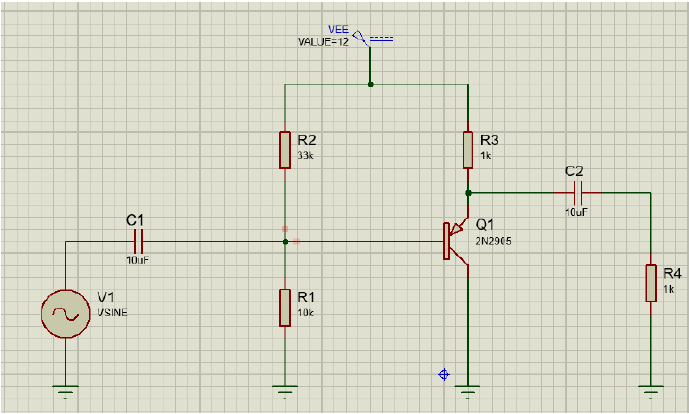
\includegraphics[width=\textwidth, height=6cm]{./images/9.12}
\end{center}
\end{figure}

\begin{figure}[H]
	\begin{center}
		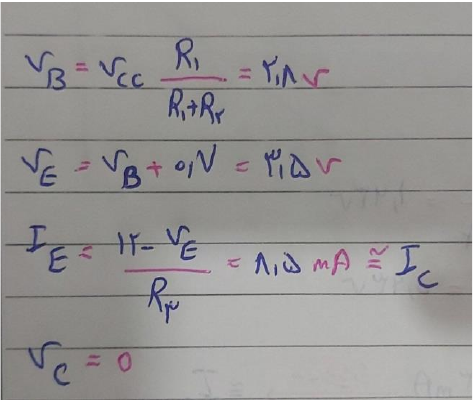
\includegraphics[width=\textwidth, height=6cm]{./images/9.12.1}
	\end{center}
\end{figure}

\begin{latin}
\begin{table}[H]
\begin{center}
\begin{tabular}{|c|c|c|}
\hline
DC \rl{پارامتر} & \rl{محاسبه شده} & \rl{اندازه‌گیری شده} \\
\hline
\hline
$V_B$ & 2.8 & 3.31 \\
\hline
$V_E$ & 3.5 & 4.03 \\
\hline
$I_E$ & 0.0085 & - \\
\hline
$V_c$ & 0 & 0  \\
\hline
$\beta$ & - & 131.7 \\
\hline
\end{tabular}
\end{center}
\end{table}
\end{latin}

\clearpage
\section{7}
\begin{figure}[H]
\begin{center}
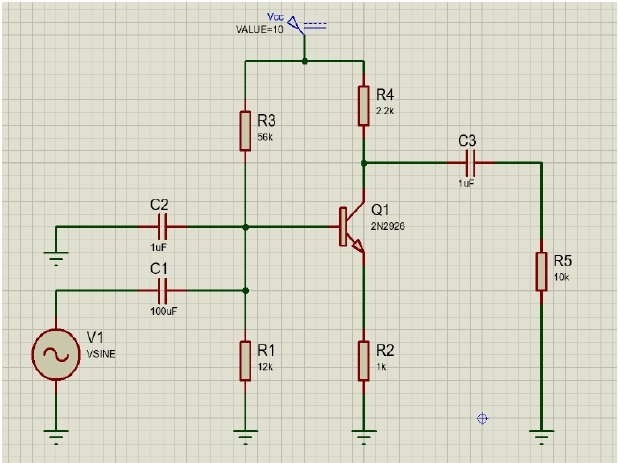
\includegraphics[width=\textwidth, height=6cm]{./images/9.13}
\end{center}
\end{figure}

\begin{figure}[H]
	\begin{center}
		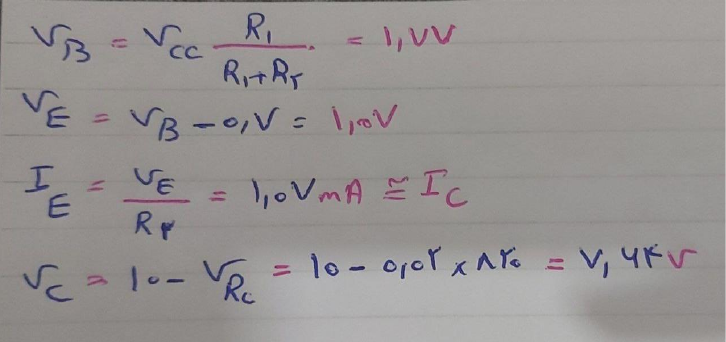
\includegraphics[width=\textwidth, height=6cm]{./images/9.13.1}
	\end{center}
\end{figure}

\begin{latin}
\begin{table}[H]
\begin{center}
\begin{tabular}{|c|c|c|}
\hline
DC \rl{پارامتر} & \rl{محاسبه شده} & \rl{اندازه‌گیری شده} \\
\hline
\hline
$V_B$ & 1.77 & 1.72 \\
\hline
$V_E$ & 1.07 & 10.5 \\
\hline
$I_E$ & 0.00107 & - \\
\hline
$V_c$ &7.646 & 7.68 \\
\hline
$\beta$ & - & 274.151 \\
\hline
\end{tabular}
\end{center}
\end{table}
\end{latin}

\end{document}